\documentclass[12pt]{article}

\usepackage[margin=1.0in]{geometry}
\usepackage[links,assignheader]{assign}
\usepackage{parskip}

\title{Acma 490 Exercises}
\author{Nathan Esau}
\date{\today}

\lhead{Acma 490 Exercises \\ Spring 2017}
\rhead{Nathan Esau \\ 301197568}

\numberwithin{questioncounter}{section}

\usepackage{Sweave}
\begin{document}
\Sconcordance{concordance:LifeInsuranceContracts.tex:LifeInsuranceContracts.Rnw:%
1 15 1 1 0 110 1 1 2 1 0 4 1 1 3 1 0 1 3 1 0 1 2 3 0 1 2 49 1 1 2 1 0 1 %
2 1 1 1 2 1 1 1 2 1 1 1 5 3 0 1 3 1 0 1 3 4 0 1 2 65 1 1 3 2 0 1 2 1 0 %
1 2 1 0 1 3 4 0 1 2 2 1 1 16 15 0 1 16 14 0 1 2 1 1 3 0 1 2 9 1 1 2 1 0 %
1 1 3 0 1 2 28 1 1 3 2 0 1 3 2 0 1 2 1 3 4 0 1 2 8 1 1 2 1 0 1 1 1 3 1 %
0 1 1 1 2 1 11 9 0 1 16 17 0 1 2 181 1 1 3 2 0 1 2 1 1 1 2 1 1 1 2 1 1 %
3 0 1 2 60 1}


\maketitle

\thispagestyle{empty}

\tableofcontents

\newpage

\setcounter{section}{1}
\section{Deterministic interest (Pure insurance risk)}

\begin{question}
Find $E[Z_{k+1}]$ and $Var[Z_{k+1}]$ for a whole-life insurance payable at the end of the year of death if the future lifetime of the life insured is exponentially distributed with parameter $\mu$ (mean $1/\mu$). Use a constant force of interest of $\delta$.
\end{question}

\begin{solution}
Since ${}_{k|}q_{x} = {}_{k}p_{x} + {}_{k+1}p_{x} = e^{-\mu k} - e^{-\mu(k+1)} = e^{-\mu k} (1 - e^{-\mu})$ we have that

\begin{align*}
E[Z_{k+1}] &= \sum_{k=0}^{\infty} e^{-\delta k} e^{-\delta} (1 - e^{-\mu}) e^{-\mu k} \\
&= \sum_{k=0}^{\infty} e^{-k(\delta + \mu)} (1 - e^{-\mu}) e^{-\delta} \\
&= \dfrac{1}{1 - e^{-(\delta + \mu)}} (1 - e^{-\mu}) e^{-\delta}
\end{align*}

The second moment is

\begin{align*}
E[Z_{k+1}^{2}] &= \sum_{k=0}^{\infty} e^{-2\delta k} e^{-2\delta} (1 - e^{-\mu}) e^{-k(2\delta + u)} \\
&= \dfrac{1}{1 - e^{-(2\delta + \mu)}} (1 - e^{-\mu}) e^{-2\delta}
\end{align*}

\end{solution}

\begin{question}
Find $A_{x}$ and $Var[Z_{k+1}]$ if ${}_{k|}q_{x}= pq^{k}$ for $k = 0, 1, 2, \dots, \infty$. Compare with question 2.1.
\end{question}

\begin{solution}
The first moment is

\begin{align*}
E[Z_{k+1}] &= \sum_{k=0}^{\infty} {}_{k|}q_{x} \exp\left(-\delta(k+1)\right) \\
&= \sum_{k=0}^{\infty} pq^{k} (e^{-\delta(k)}) e^{-\delta} \\
&= \dfrac{pe^{-\delta}}{1 - qe^{-\delta}}
\end{align*}

Note that this is the same as in Exercise 2.1 if $p = (1 - e^{-\mu})$ and $q = e^{-\mu}$. The second moment is

\begin{align*}
E[Z_{k+1}^{2}] &= \sum_{k=0}^{\infty} e^{-2\delta} p(qe^{-2\delta})^{k} \\
&= \dfrac{pe^{-2\delta}}{1- qe^{-2\delta}}
\end{align*}

\end{solution}

\begin{question}
Using De Moivre ($l_{x} = l_{0} (1 - x/\omega)$ for $0 < x < \omega$), find $E[Z_{k+1}]$ and $Var[Z_{k+1}]$ for a discrete whole-life insurance.
\end{question}

\begin{solution}
For $T_{x} \sim U(0, \omega - x)$ so ${}_{k|}q_{x} = \dfrac{1}{\omega - x}$ and we have that

\begin{align*}
E[Z_{k+1}] &= \sum_{k=0}^{\omega - x - 1} {}_{k|}q_{x} e^{-\delta k} \\
&= \sum_{k=0}^{\omega - x - 1} \dfrac{1}{\omega - x} e^{-\delta k} \\
&= \dfrac{1 - e^{-\delta (\omega - x)}}{(\omega - x) (1 - e^{-\delta})}
\end{align*}

and the second moment is

\begin{align*}
E[Z_{k+1}^{2}] &= \sum_{k=0}^{\omega - x - 1} \dfrac{1}{\omega - x} e^{-2\delta k} \\
&= \dfrac{1 - e^{-2\delta (\omega - x)}}{(\omega - x)(1 - e^{-2\delta})}
\end{align*}

\end{solution}

\begin{question}
Consider 100 independent lives insured aged $x$, subject to a constant force of mortality ($\mu = 0.04$) and all covered by a single premium 10-year temporary insurance contract of \$2,000,000 payable at the end of the year of death (if within 10 years, of course). The death benefits will be paid from a fund earning $\delta = 0.06$. Calculate the amount needed in that fund at time 0 such that the probability of being able to pay all the benefits is 0.95.
\end{question}

\begin{solution}
The first moment is

\begin{align*}
E[Z(c)] &= c \times  \dfrac{b e^{-\delta} (1 - e^{-\mu}) (1 - e^{-(\delta + \mu)n})}{1 - e^{-(\delta + \mu)}}
\end{align*}

The second moment is

\begin{align*}
E[Z(c)^2] &= c^2 \times  \dfrac{b^2 e^{-2 \delta} (1 - e^{-\mu}) (1 - e^{-(2 \delta + \mu)n})}{1 - e^{-(2 \delta + \mu)}}
\end{align*}

The variance is

\begin{align*}
Var[Z(c)] &= c^{2} \left\{ E[Z(c)^2] - E[Z(c)]^{2} \right\}
\end{align*}

Using the normal approximation, the amount needed is

\begin{align*}
1.645 \sqrt{Var[Z(c)]} + E[Z(c)]
\end{align*}

This is calculated using R below.

\begin{Schunk}
\begin{Sinput}
> mu = 0.04
> delta = 0.06
> n = 10
> b = 2e+06
> c = 100
> first = b * exp(-delta) * (1 - exp(-mu)) * (1 - exp(-(delta + mu)*n)) / 
+ 	(1 - exp(-(delta + mu)))
> second = b^2 * exp(-2*delta) * (1 - exp(-mu)) * 
+ 	(1 - exp(-(2*delta + mu)*n)) / (1 - exp(-(2*delta + mu)))
> amount = 1.645 * sqrt(c * (second - first^2)) + first * c
\end{Sinput}
\end{Schunk}

This gives an amount of $60807943$.

\end{solution}

\begin{question}
Show that $Var[Z(c)]$ obtained from using the result for the variance of iid random variables is equivalent to using (2.8) and (2.9).
\end{question}

\begin{solution}
%Using (2.8) and (2.9), we have that

%\begin{align*}
%Var[Z(c)] &= E[Z(c)^2] - E[Z(c)]^2 \\
%&= c(c-1)E[Z_{1}Z_{2}] + c E[Z_{1} Z_{1}] - c^2E[Z_{1}]^2 \\
%&= c(c-1)E[Z^2] + cE[Z^2] - c^{2}E[Z]^2 \\
%&= c^{2}E[Z^{2}] - c^{2}E[Z]^{2}
%\end{align*}

Using first principles, the variance of $Z(c)$ is

\begin{align*}
Var[Z(c)] &= Var\left[\sum_{i=1}^{c} Z_{i} \right] \\
&= \sum_{i=1}^{c} Var[Z_{i}] \\
&= c [E[Z^2] - E[Z]^2]
\end{align*}

\end{solution}

\begin{question}
Find an expression for $E[Z_{1}^{2}Z_{2}]$.
\end{question}

\begin{solution}
We have that

\begin{align*}
E[Z_{1}^{2}Z_{2}] &= \sum_{k_{1}} \sum_{k_{2}} (b_{k_{1} + 1} v^{k_{1} + 1})^2 b_{k_{2} + 1} v^{k_{2} + 1} {}_{k_{1}|}q_{x} {}_{k_{2}|}q_{x}
\end{align*}

\end{solution}

\begin{question}
Rework section 2 for $n$-year endowment contracts.
\end{question}

\begin{solution}

The functions used for the endowment insurance are shown below.

\begin{Schunk}
\begin{Sinput}
> library(stocins) # see github.com/nathanesau
> irm = iratemodel(list(delta = 0.06), "determ")
> mort = mortassumptions(list(x=50, table="MaleMort82"))
> endow1 = insurance(list(n = 1, d = 1, e = 1), "isingle", "endow")
> endow10 = insurance(list(n = 10, d = 1, e = 1), "isingle", "endow")
> port1 = insurance(list(single = endow1, c = 10), "iport", "endow")
> port10 = insurance(list(single = endow10, c = 10), "iport", "endow")
> first = c(z.moment(1, endow1, mort, irm),
+ 	z.moment(1, endow10, mort, irm),
+ 	z.moment(1, port1, mort, irm) / port1$c,
+ 	z.moment(1, port10, mort, irm) / port1$c)
> sdev = c(0, z.sd(endow10, mort, irm), 0, 
+ 	z.sd(port10, mort, irm) / port1$c)
> skew = c(0, z.sk(endow10, mort, irm),
+ 	0, z.sk(port10, mort, irm))
\end{Sinput}
\end{Schunk}

\begin{table}[ht]
\begin{center}
\begin{tabular}{l r r r r}
\hline
$c$ & $n$ & $E[Z(c)/c]$ & $sd[Z(c)/c]$ & $sk[Z(c)/c]$ \\ \hline
1 & 1 & 0.94176 & 0 & 0 \\
1 & 10 & 0.56337 & 0.0582 & 4.57037 \\
10 & 1 & 0.94176 & 0 & 0 \\
10 & 10 & 0.56337 & 0.01841 & 1.44528 \\ \hline
\end{tabular}
\end{center}
\end{table}

\end{solution}

\newpage

\setcounter{section}{2}
\section{Life Insurance with Random Interest and Mortality}

\begin{question}
It has been suggested that the interest rate risk and the mortality risk can be studied independently since $K$ and $\delta$ are assumed independent. More precisely, the suggestion is that the total ``uncertainty'' in $Z$ is the sum of

\begin{enumerate}[(i)]
\item the variance of the random discounted values when the mortality is assumed to follow exactly the life table, and
\item the variance of the present value of the benefit discounted at the deterministic expected interest rates
\end{enumerate}

\begin{enumerate}[(a)]
\item Formulate this mathematically for a temporary insurance contract.
\item Illustrate the approach with a 10-year temporary insurance contract issued to someone aged 50, using an Ornstein-Uhlenbeck process with $\delta = 0.05$, $\delta_{0} = 0.08$, $\alpha = 0.1$ and $\sigma = 0.02$. (Find the variance of $Z$, the interest rate risk and the mortality risk).
\item Compare the numerical results given by the 2 components of (3.16).
\item Redo this problem when (ii) above is replaced by the variance of the present value of the benefit discounted at the deterministic expected discount factors, $E[e^{-y(t)]}]$.
\end{enumerate}

\end{question}

\begin{solution}

\begin{enumerate}[(a)]
\item Formulas for the two components are derived below.

\begin{enumerate}[(i)]
\item The investment risk is

\begin{align*}
Var_{y} \left[\sum_{k} {}_{k|}q_{x} e^{-y(k+1)}\right]
\end{align*}

\item The insurance risk is

\begin{align*}
Var_{k}[e^{-\delta(k+1)}]
\end{align*}

\end{enumerate}

\item The $m$th moment of $Z$ is

\begin{align*}
E[Z^{m}] &= \sum_{k=0}^{n-1} E[e^{-my(k+1)}] {}_{k|}q_{x}
\end{align*}

from which we can easily calculate the variance of $Z$. This is done using R below.

\begin{Schunk}
\begin{Sinput}
> mort = mortassumptions(params = list(x = 50, 
+ 	table = "MaleMort82"))
> oumodel = iratemodel(params = list(delta = 0.05, 
+ 	delta0 = 0.08, alpha = 0.10, sigma = 0.02), "ou")
> term = insurance(params = list(n = 10, d = 1), 
+ "isingle", "term")
> VarZ = z.moment(2, term, mort, oumodel) - 
+   z.moment(1, term, mort, oumodel)^2    
\end{Sinput}
\end{Schunk}
 
Some functions to calculate the two components are shown below. 
  
\begin{Schunk}
\begin{Sinput}
> insrisk <- function(ins, mort, irm)
+ {
+   second = 0
+   first = 0
+   
+   for(k in seq(0,ins$n-1,1))
+   {
+     second = second + exp(-y.ev(k+1,irm)*2) * 
+     kdeferredqx(k, mort)
+     first = first + exp(-y.ev(k+1,irm)) * 
+     kdeferredqx(k, mort)
+   }
+   
+   second - first^2
+ }
> invrisk <- function(ins, mort, irm)
+ {
+   total = 0
+   
+   for(k in seq(0,ins$n-1,1))
+   {
+     for(j in seq(0,ins$n-1,1))
+     {
+       total = total + pv.cov(k+1,j+1,irm) * kdeferredqx(k,mort) * 
+       kdeferredqx(j, mort)
+     }
+   }
+   
+   total
+ }
> InsuranceRisk = insrisk(term, mort, oumodel)
> InvestmentRisk = invrisk(term, mort, oumodel)
\end{Sinput}
\end{Schunk}

This gives $Var[Z] = 0.04069478$.

\begin{enumerate}[(i)]
\item The variance of the random discounted values is $6.753e-05$.
\item The variance of the present value of the benefit is $0.03901077$.
\end{enumerate}

\item The components of 3.16 are calculated below.

\begin{Schunk}
\begin{Sinput}
> InsuranceRisk = z.insrisk(term, mort, oumodel)
> InvestmentRisk = z.invrisk(term, mort, oumodel)
\end{Sinput}
\end{Schunk}

This gives

\begin{enumerate}[(i)]
\item The insurance risk is $0.00090981$.
\item The investment risk is $0.03978498$.
\end{enumerate}

\item Omit

\end{enumerate}

\end{solution}

\begin{question}
Modeling the force of interest by an Ornstein-Uhlenbeck process with $\delta = 0.05$, $\delta_0 = 0.03$, $\alpha = 0.1$ and $\sigma = 0.02$, study the discount function, $e^{-y(t)}$.

\begin{enumerate}[(a)]
\item For which value of $t$ is its standard deviation (or variance) maximum?
\item Calculate the standard deviation of $Z$ for temporary insurance contracts for different values of $n$ and $x$. Referring to section 3.2, could you have ``roughly predicted'' those results?
\end{enumerate}

\end{question}

\begin{solution}

\begin{enumerate}[(a)]
\item The graph is shown below. The maximum variance occurs for $t = 39.7624$.

\begin{Schunk}
\begin{Sinput}
> oumodel = iratemodel(params = list(delta = 0.05, delta0 = 0.03, 
+ 	alpha = 0.10, sigma = 0.02), "ou")
> pv.var <- function(t) {
+ 	pv.moment(t,2,oumodel) - pv.moment(t,1,oumodel)^2
+ }
> plot(pv.var, 0, 100, ylab = "Var[pv(t)]", xlab = "t")
> maxt = optim(par=c(20), fn=function(t)-pv.var(t),
+              method="Brent", lower=0, upper=50)$par
\end{Sinput}
\end{Schunk}

\begin{figure}[ht]
\begin{center}
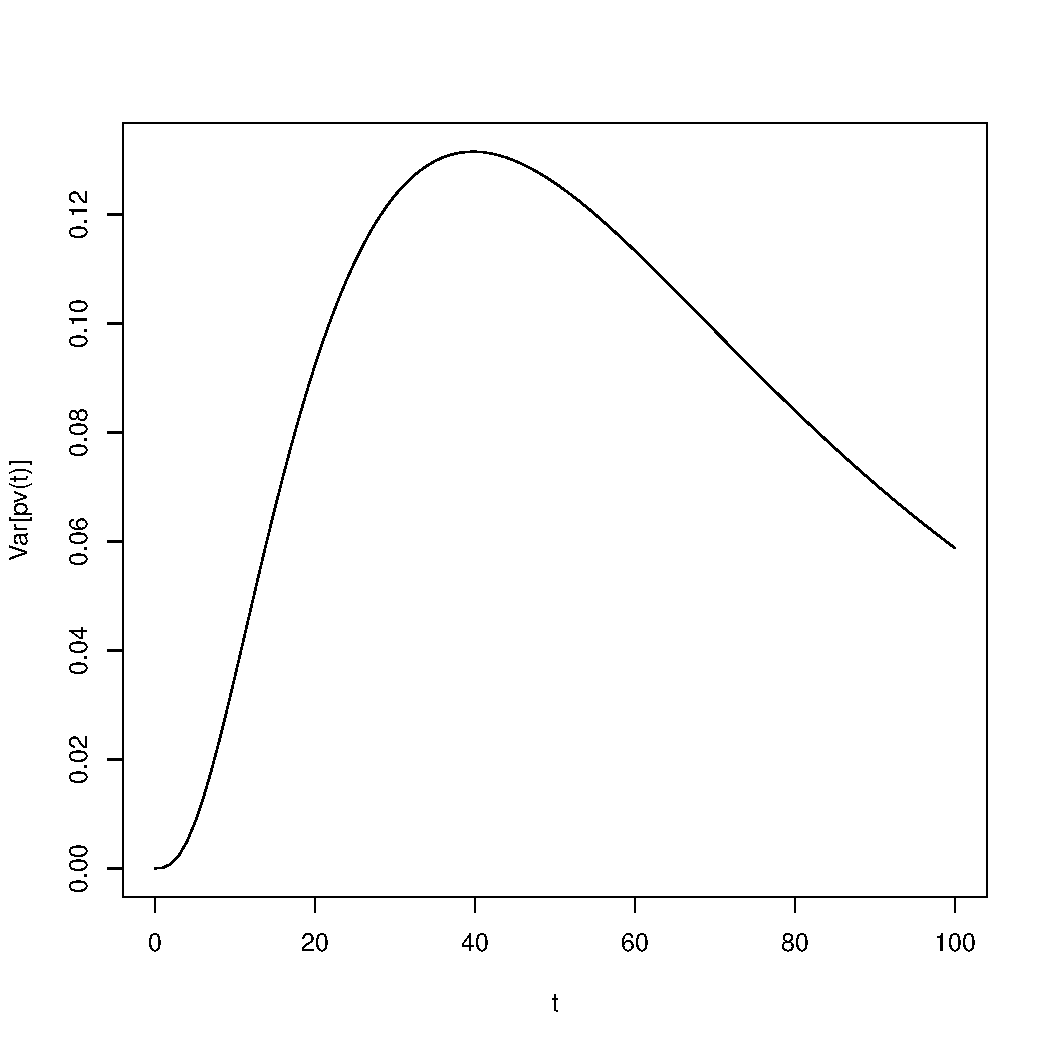
\includegraphics[width=0.7\textwidth]{images/exercise32_1}
\end{center}
\end{figure}

\item The graph is shown below.

\begin{Schunk}
\begin{Sinput}
> library(lattice)
> library(latex2exp)
> # tweak g params
> g <- expand.grid(y = seq(1,70,20), x = seq(20,70,25))
> g$z <- numeric(nrow(g))
> counter = 1
> for(i in 1:nrow(g))
+ {
+   term = insurance(params = list(n = g$y[counter], d = 1), 
+   "isingle", "term")
+   mort = mortassumptions(params = list(x = g$x[counter], 
+   table = "MaleMort82"))
+   
+   g$z[counter] = z.sd(term, mort, oumodel)
+   counter = counter + 1
+ }
> wireframe(z ~ y * x, data = g,
+           drape = TRUE,
+           col = 'black',
+           col.regions = 'white',
+           aspect = c(1.0, 0.8),
+           colorkey = FALSE,
+           xlab = "n",
+           ylab = "issue age",
+           zlab = "",
+           screen = list(z = 340, x = -70),
+           scales = list(arrows = FALSE, col="black", font = 10,
+                         cex= 1.0),
+           par.settings = list(regions=list(alpha = 0.3),
+                               axis.line = list(col = "transparent")),
+           zoom = 0.90)
\end{Sinput}
\end{Schunk}

\begin{figure}[ht]
\begin{center}
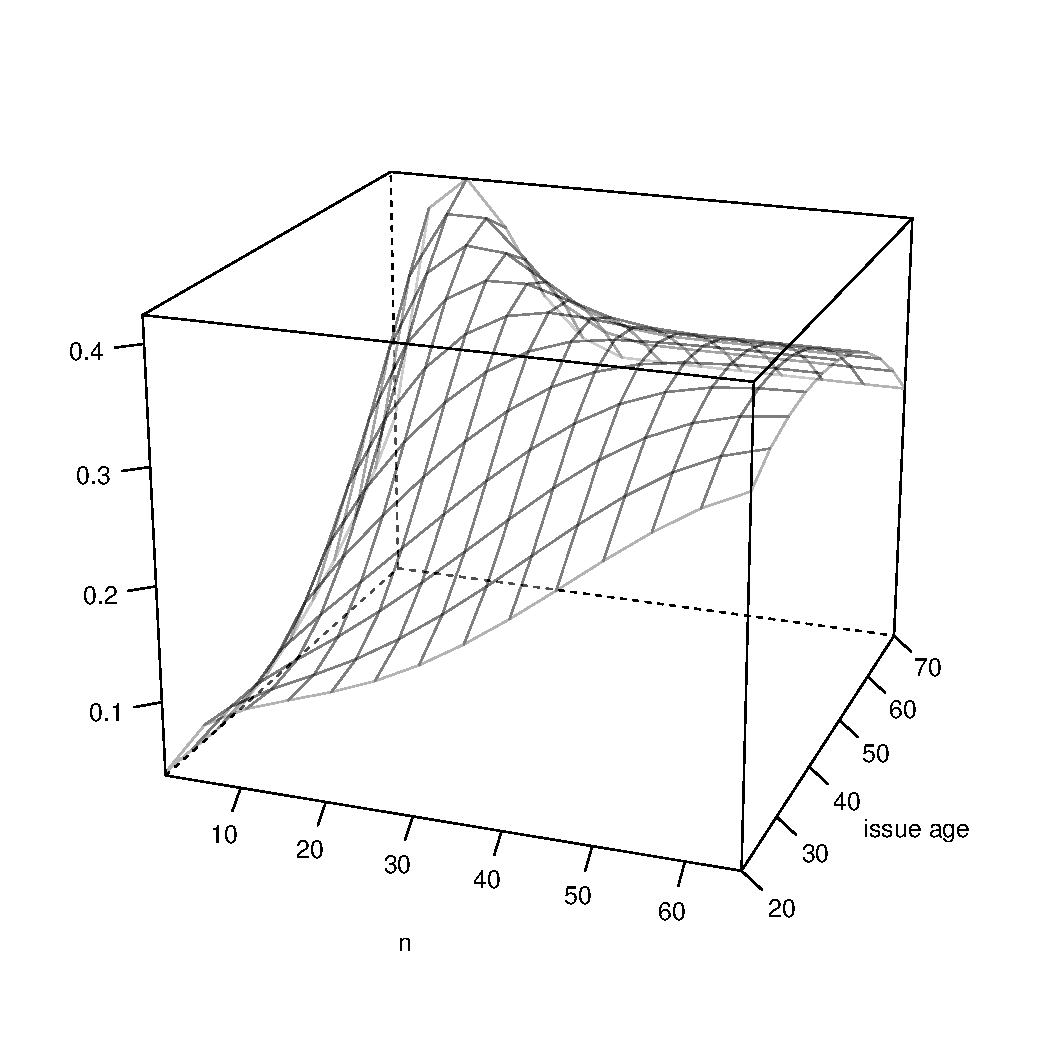
\includegraphics[width=0.9\textwidth]{images/exercise32}
\end{center}
\vspace{-15mm}
\caption{Standard deviation for Exercise 3.2}
\end{figure}

\end{enumerate}

\end{solution}

\newpage

\setcounter{section}{3}
\section{A Portfolio of Policies with Random Interest and Mortality}

\begin{question}
Prove (4.10).
\end{question}

\begin{solution}
We have that

\begin{align*}
E[Z(c)^2] &= c(c-1)E[Z_{1}Z_{2}] + cE[Z^2] \\
E[Z(c)]^{2} &= c^2 E[Z]^2
\end{align*}

so the variance per policy is

\begin{align*}
\dfrac{Var[Z(c)]}{c^2} &= \dfrac{c(c-1)}{c^2} E[Z_{1}Z_{2}] + \dfrac{cE[Z^2]}{c^2} - \dfrac{c^2}{c^2} E[Z]^2
\end{align*}

and the limiting variance is

\begin{align*}
\lim_{c \to \infty} \dfrac{Var[Z(c)]}{c^2} &= E[Z_{1}Z_{2}] - E[Z]^2
\end{align*}

\end{solution}

\begin{question}
\begin{enumerate}[(a)]
\item Show that $\dfrac{d}{dc} Var[Z(c)/c] = - \dfrac{1}{c^2} ({}^{2}A - E[Z_{1}Z_{2}])$ if it is treated as a continuous function of $c$.

\item Show that under assumptions 4.2, the above derivative if $-E[Var(Z|y(t))]/c^2$
\end{enumerate}
\end{question}

\begin{solution}
\begin{enumerate}[(a)]
\item Using the expression for $Var[Z(c)]$ from Exercise 4.1,

\begin{align*}
\dfrac{Var[Z(c)]}{c^2} &= \dfrac{c(c-1)}{c^2} E[Z_{1}Z_{2}] + \dfrac{cE[Z^2]}{c^2} - \dfrac{c^2}{c^2} E[Z]^2 \\
&= (1 - c^{-1}) E[Z_{1}Z_{2}] + \dfrac{1}{c} E[Z^2] - E[Z]^2
\end{align*}

so the derivative is

\begin{align*}
\dfrac{d}{dc} \dfrac{Var[Z(c)]}{c^2} &= c^{-2} E[Z_{1}Z_{2}] - c^{-2} E[Z^2] \\
&= -\dfrac{1}{c^2} [-E[Z_{1}Z_{2}] + E[Z^2]]
\end{align*}

\item Using the result of (a), we just need to show that

\begin{align*}
E[Var[Z | \{y(t)\}]] &= E[Z^2] - E[Z_{1}Z_{2}]
\end{align*}

using Equation (4.8) we have that

\begin{align*}
E[Var[Z|\{y(t)\}]] &= E\Big[ E[Z^2|\{y(t)\}] - E[Z|\{y(t)\}] \cdot E[Z|\{y(t)\}] \Big] \\
&= E[Z^2] - E\Big[ E[Z_{1}|\{y(t)\}] \cdot E[Z_{2}|\{y(t)\}] \Big] \\
&= E[Z^2] - E\Big[ E[Z_{1}Z_{2}|\{y(t)\}] \Big] \\
&= E[Z^{2}] - E[Z_{1}Z_{2}]
\end{align*}

\end{enumerate}
\end{solution}

\begin{question}
Prove (4.20).
\end{question}

\begin{solution}
The third central moment is

\begin{align*}
\dfrac{E[Z(c)^{3}]}{c^3} - \dfrac{3E[Z(c)^2]E[Z(c)]}{c^3} + \dfrac{2E[Z(c)]^{3}}{c^3}
\end{align*}

The limit for each of these terms is

\begin{align*}
\lim_{c\to \infty} \dfrac{E[Z(c)^3]}{c^3} &= \dfrac{c(c-1)(c-2)E[Z_{1}Z_{2}Z_{3}]}{c^3} + \dfrac{3c(c-1)E[Z_{1}^{2}Z_{c}]}{c^3} + \dfrac{cE[Z^{3}]}{c^3} \\
&= E[Z_{1}Z_{2}Z_{3}] \\
\lim_{c \to \infty} \dfrac{E[Z(c)^2]E[Z(c)]}{c^3} &= \dfrac{c(c-1)E[Z_{1}Z_{2}]cE[Z]}{c^3} + \dfrac{cE[Z^{2}]cE[Z]}{c^3} \\
&= E[Z_{1}Z_{2}] \\
\lim_{c\to \infty} \dfrac{E[Z(c)]^{3}}{c^3} &= \dfrac{c^{3}E[Z^{3}]}{c^3} \\
&= E[Z^{3}]
\end{align*}

so the limit of the third central moment is

\begin{align*}
\lim_{c \to \infty} \dfrac{E[Z(c)^{3}]}{c^3} - \dfrac{3E[Z(c)^2]E[Z(c)]}{c^3} + \dfrac{2E[Z(c)]^{3}}{c^3} &= E[Z_{1}Z_{2}Z_{3}] - 3E[Z_{1}Z_{2}] + 2E[Z^3]  
\end{align*}

from Exercise 4.1, $\lim_{c\to \infty} Var[Z(c)]/c^2 = E[Z_{1}Z_{2}] - E[Z^{2}]$ so the limiting skewness is

\begin{align*}
\lim_{c\to \infty} sk[Z(c)/c] &= \dfrac{E[Z_{1}Z_{2}Z_{3}] - 3E[Z_{1}Z_{2}] + 2E[Z^3]}{(E[Z_{1}Z_{2}] - E[Z^{2}])^{3/2}}
\end{align*}

\end{solution}

\begin{question}
\begin{enumerate}[(a)]
\item Show that for $n$-year temporary insurance contracts
%
\begin{align*}
\lim_{c \to \infty} Var[Z(c)/c] &= \sum_{k_{1} = 0}^{n-1} \sum_{k_{2} = 0}^{n-1} {}_{k_{1}|}q_{x} \cdot {}_{k_{2}|}q_{x} cov(e^{-y(k_{1} + 1)}, e^{-y(k_{2} + 1)})
\end{align*}

\item Show that this limiting variance is increasing with $n$.

\end{enumerate}
\end{question}

\begin{solution}

\begin{enumerate}[(a)]
\item The variance is

\begin{align*}
\dfrac{Var[Z(c)]}{c^2} &= \dfrac{c(c-1)}{c^2} \sum_{k_{1}=0}^{n - 1} \sum_{k_{2} = 0}^{n - 1} E[e^{-y(k_{1} + 1) - y(k_{2} + 1)}] {}_{k_{1}|}q_{x} {}_{k_{2}|}q_{x} + \dfrac{c}{c^2} \sum_{k=0}^{n - 1} E[e^{-y(k+1)^2}] {}_{k|}q_{x} \ - \\
&\qquad \dfrac{c^2}{c^{2}} \left[ \sum_{k=0}^{n-1} E[e^{-y(k+1)}] {}_{k|}q_{x} \right]^{2}
\end{align*}

so the limiting variance is

\begin{align*}
\lim_{c\to \infty} \dfrac{Var[Z(c)]}{c^2} &= \sum_{k_{1}=0}^{n-1} \sum_{k_{2} = 0}^{n-1} E[e^{-y(k_{1} + 1) - y(k_{2} + 1)}] {}_{k_{1}|}q_{x} {}_{k_{2}|}q_{x} - \sum_{k=0}^{n-1} E[e^{-y(k+1)}]^{2} {}_{k|}q_{x}^{2}
\end{align*}

The covariance of two present values is

\begin{align*}
Cov[e^{-y(k_{1} + 1)}, e^{-y(k_{2} + 1)}] &= E[e^{-y(k_{1} + 1) - y(k_{2} + 1)}] - E[e^{-y(k_{1} + 1)}]  E[e^{-y(k_{2} + 1)}]
\end{align*}

we can rearrange the limiting variance, i.e.

\begin{align*}
\lim_{c \to \infty} \dfrac{Var[Z(c)]}{c^2} &= \sum_{k_{1}=0}^{n-1} \sum_{k_{2} = 0}^{n-1} E[e^{-y(k_{1} + 1) - y(k_{2} + 1)}] {}_{k_{1}|}q_{x} {}_{k_{2}|}q_{x}  \ - \\
&\qquad \sum_{k_{1} = 0}^{n-1} E[e^{-y(k+1)}] {}_{k_{1}|}q_{x} \sum_{k_{2} = 0}^{n-1} E[e^{-y(k_{2} + 1)}]{}_{k_{2}|}q_{x} \\
&= \sum_{k_{1}=0}^{n-1} \sum_{k_{2} = 0}^{n-1} {}_{k_{1}|}q_{x} {}_{k_{2}|}q_{x} cov[pv(k_{1}+1), pv(k_{2}+1)]
\end{align*}

\end{enumerate}

\end{solution}

\begin{question}
\begin{enumerate}[(a)]
\item Calculate the standard deviation of $Z(c)/c$ for $c = 10$ and $\infty$ for the 10-year temporary insurance contract of exercise 3.1 (b).
\item Is the limiting variance equal to the interest risk defined in (3.17)? Is it equal to component (1) in exercise 3.1?
\end{enumerate}
\end{question}

\begin{solution}

\begin{enumerate}[(a)]

\item The following additional code to exercise 3.1 (b) was needed to calculate $sd[Z(c)/c]$.

\begin{Schunk}
\begin{Sinput}
> oumodel = iratemodel(list(delta = 0.05, delta0 = 0.08,
+ 	alpha = 0.10, sigma = 0.02), "ou")
> mort = mortassumptions(list(x = 50, table = "MaleMort82"))	
> term = insurance(list(n = 10, d = 1), "isingle", "term")
> port10 = insurance(list(single = term, c = 10), "iport", "term")
> portInf = insurance(list(single = term, c = 1e18), "iport", "term")
> sd10 = z.sd(port10, mort, oumodel) / port10$c
> sdInf = z.sd(portInf, mort, oumodel) / portInf$c
\end{Sinput}
\end{Schunk}

This gives $sd[Z(c)/c] = 0.06426706$ for $c = 10$ and $sd[Z(c)/c] = 0.0082176$ for $c = \infty$.

\item The limiting variance is $6.753e-05$. This is the same as component (1) in exercise 3.1.

\end{solution}

\setcounter{section}{4}

\newpage

\section{Distribution of the Present Value of Benefits for a Portfolio}

\begin{question}
\begin{enumerate}[(a)]
\item Show that $\rho(y(n), y(n-1))$ does not depend on the parameters of the White Noise process for the force of interest.
\item Show that $\rho(y(n), y(n-1))$ does not depend on the parameters $\delta$, $\delta_{0}$ and $\sigma$ of the Ornstein-Uhlenbeck process for the force of interest.
\end{enumerate}
\end{question}

\begin{solution}

\begin{enumerate}[(a)]
\item For a white-noise process, $Var[y(t)] = \sigma^{2} t$ and $Cov[y(s), y(t)] = \sigma^{2} \min(s,t)$ so we have that

\begin{align*}
\rho(y(n), y(n-1)) &= \dfrac{Cov(y(n), y(n-1)}{\sqrt{Var(y(n))}\sqrt{Var(y(n-1))}} \\
&= \dfrac{\sigma^{2} (n-1)}{\sqrt{\sigma^{2} n}\sqrt{\sigma^{2} (n-1)}} \\
&= \dfrac{(n-1)}{[n(n-1)]^{0.5}}
\end{align*}

this does not depend on $\sigma^2$.

\item For an Ornstein-Uhlenbeck process, 

\begin{align*}
Var[y(t)] &= \dfrac{\sigma^2}{\alpha^2} t + \dfrac{\sigma^2}{2\alpha^3} (-3 + 4\exp(-\alpha t) - \exp(-2\alpha t)) \\
Cov[y(s), y(t)] &=  \dfrac{\sigma^2}{\alpha^2} \min(s, t) +
    \dfrac{\sigma^2}{2\alpha^3} (-2 + 2\exp(-\alpha s) + \\
    &\qquad 2\exp(-\alpha t) 
                             - \exp(-\alpha |t-s|) - \exp(-\alpha (t+s)))
\end{align*}

so we have that

{\footnotesize
\begin{align*}
\rho(y(n), y(n-1)) &= \dfrac{\dfrac{\sigma^2}{\alpha^2} (n-1) +
    \dfrac{\sigma^2}{2\alpha^3} (-2 + 2e^{-\alpha (n-1)} + 2e^{-\alpha (n)} - e^{-\alpha} - e^{-\alpha (2n - 1)})}{\sqrt{\dfrac{\sigma^2}{\alpha^2} n + \dfrac{\sigma^2}{2\alpha^3} (-3 + 4e^{-\alpha n} - e^{-2\alpha n})}\sqrt{\dfrac{\sigma^2}{\alpha^2} (n-1) + \dfrac{\sigma^2}{2\alpha^3} (-3 + 4e^{-\alpha (n-1)} - e^{-2\alpha (n-1)})}} \\
&= \dfrac{\dfrac{1}{\alpha^2} (n-1) +
    \dfrac{1}{2\alpha^3} (-2 + 2e^{-\alpha (n-1)} + 2e^{-\alpha (n)} - e^{-\alpha} - e^{-\alpha (2n - 1)})}{\sqrt{\dfrac{1}{\alpha^2} n + \dfrac{1}{2\alpha^3} (-3 + 4e^{-\alpha n} - e^{-2\alpha n})}\sqrt{\dfrac{1}{\alpha^2} (n-1) + \dfrac{1}{2\alpha^3} (-3 + 4e^{-\alpha (n-1)} - e^{-2\alpha (n-1)})}}
\end{align*}
}

which only depends on $\alpha$.

\end{enumerate}

\end{solution}

\end{document}
